One of the earliest and most comprehensive definitions of information retrieval (IR) is by Salton (1968)~\cite{salton-1968}, which describes IR to be a field encompassing the structure, analysis, organization, storage, searching and retrieval of information. It has been primarily focused on large-scale unstructured textual data, such as web pages, but it could involve any type of data \cite{ir-in-practise}. Programming language code is considered as unstructured data although, in comparison to text or web pages, it has very formal grammar and the tokens it allows are very limited.

In our case we are interested in finding the most relevant student submissions given teacher's information need but translating these needs into particular information retrieval objectives is tricky. Our assumption is that the two most important ones are to find outliers from the dataset and also to divide it into structurally distinctive clusters. Still, these goals are not specific enough to exactly model the actual retrieval process from the user interface all the way to the used data format.

As a general description of an IR process, a user has an information need which they try to describe using a search interface of an IR system. The system executes the user's search query and returns the most relevant documents which would satisfy that need. For our educational search, the process could utilize various data as part of the retrieval, such as the number of attempted tests or the historical performance of the student, yet to simplify the scope of the research we shall only consider submitted code which has passed the tests and therefore is assumed to be correct.

Next, the most common IR system, the search engine, is described and the different IR representation models it could use. Set-theoretic models are the most simplistic models that filter the documents by marking them either \texttt{true} or \texttt{false} given search query without ranking the documents by their relevancy scores. Algebraic models allow the ranking of the documents but they are constrained to the specific ranking algorithm they use. Probabilistic models offer a more flexible approach to model the uncertainty of relevancy in their scoring but which might result in more complicated and slower models \cite{intro-to-ir, ir-in-practise}.

As this thesis does not aim to research how to construct a custom search engine for code, the research of the IR techniques is left to a general overview. The focus of the research is aimed towards the algebraic vector space model as it is a flexible method that can also be used for other purposes, and which CodeClusters uses for its similarity detection n-gram model. The main takeaways from choosing an IR model is that regardless of the model, a good weighting and similarity scoring mechanism is crucial for producing the most relevant results. A poor weighting and similarity measure will not be able to distinguish between documents of varying size and content. The possible formats to represent program code are described in more detail in the Section~\ref{sec:representations} and the similarity scoring in the Section~\ref{sec:sim-detection}. This Section was mostly based on the books \textit{Information Retrieval in Practice} (2011) by Croft et al.~\cite{ir-in-practise} and \textit{An Introduction to Information Retrieval} (2009) by Manning et al.~\cite{intro-to-ir}.

\subsection{IR system}
\label{ssec:ir-system}

Information retrieval is, as its name states, retrieving of relevant information. But can we define it more formally? A simplistic definition could be that we have a set of documents $D=\{d_1, d_2, ..., d_n\}$ such that each contains unstructured data, often natural language text, but for us, code. We assume a pre-processing of the documents has taken place in which the text, or code, has been parsed into a sequence of terms: $d_j=[t_{1,j}, ... t_{m,j}]$. Terms are individual string tokens that represent either the original words, separated by for example whitespace, or their basic grammatical forms. Commonly stop-words like "the" or "an" are discarded in the parsing process with natural languages. Similarly, we could omit semicolons or brackets with code. For this set of documents, we have an information need that requires us to find the most documents relevant to that need to satisfy it. We can illustrate this process by assuming a search query $Q$, a binary relevancy scoring function $rel$ and an information retrieval function $I$, shown in the Equation \ref{eq:ir-func}.

\vspace{-6pt}
\begin{equation}
\label{eq:ir-func}
I(Q,D,rel)=[rel(Q, d_1), ...,  rel(Q, d_n)]
\end{equation}

where
\vspace{-12pt}

$$rel: (Q,d) \rightarrow c,\; c \in \{\text{"relevant"}, \text{"non-relevant"}\}$$
\vspace{-6pt}

The function $I$ takes as its inputs a query and a set of documents and outputs either "relevant" or "non-relevant" class for each document. An IR system could then use these results to filter the "relevant" documents from the "non-relevant".

Yet using search queries as part of the retrieval process may not be very applicable to our use case. We have not explicitly stated that the teachers must write the criteria they want to data to be grouped with and therefore we could omit the search query parameter $Q$. Also, this process assumes only two classes to exist while we could expect the classes, or clusters, to be numerous. Another interpretation of the process could be the function $S$ shown in the Equation \ref{eq:sim-matrix}.

\begin{equation}
\label{eq:sim-matrix}
S(D,sim)=
\begin{bmatrix}
    sim(d_1, d_1) & \dots & sim(d_1, d_j) & \dots & sim(d_1, d_n) \\
    \vdots & \ddots & \vdots & \ddots & \vdots \\
   sim(d_i, d_1) & \dots & sim(d_i, d_j) & \dots & sim(d_n, d_j) \\
    \vdots & \ddots & \vdots & \ddots & \vdots \\
    sim(d_n, d_1) & \dots & sim(d_n, d_j) & \dots & sim(d_n, d_n)
\end{bmatrix} \\
\medskip
\end{equation}

where
\vspace{-12pt}

$$sim : (a, b) \rightarrow [0,1]$$
\vspace{-6pt}

$S$ takes as its inputs a set of documents and a similarity scoring function $sim$, which is then executed for every document pair. It results in a similarity matrix which could be clustered to find the most similar submissions and have them shown to the teachers. This is the idea of similarity detection and which is described in length in the Section~\ref{sec:sim-detection}. While the theory of this process appears simple, the complication often arises from building a system that could execute the models efficiently with a suitable user interface. With IR systems the data is also often massive in volume and of varying quality that has to be constantly updated by a specific software - a crawler.

In the scope of this thesis we omit the software side of an IR system and focus on the theory of information retrieval. At the core of any IR system, or which has nowadays become synonymous with search engine, is the inverted index.

\textbf{Inverted index} is a data structure which stores the contents of documents as word-to-document mappings instead of the regular document-to-word mapping. The problem it is designed to solve can be easily illustrated by imagining a set of 1M documents with 500K unique terms that are spread across the documents. If we were to construct a matrix that contained the frequencies of each term in each document, a term-frequency matrix, we would arrive at a matrix of size 1M x 500K = 500B elements. In its full form, it would be unreasonably large to store in memory \cite{intro-to-ir}.

The distribution of words commonly follow Zipf's law which indicates that most of the terms do not exist in any given document. Therefore, the majority of values are zero which could amount to almost 99\% values in the matrix. This would make it more efficient to store only the non-zero values which is what the inverted index does by constructing an index of the terms and each document they appear in. Inverted index is, however, only a part of the overall IR system. It does not solve the actual execution of the models or how the data is represented. They are better described by the retrieval model, also known as IR model, which determines how the ranking of the documents and search queries are computed.

\iffalse
other things: search tree (binary tree), hashing, stemming, wildcards, compression

ranked Boolean retrieval
\fi

\textbf{Set-theoretic models} are IR models that treat the query process as a set-theoretic problem. Its assumption is that given a set of documents a subset can be found of the documents that are relevant to the search query. To subset the documents, set-theoretic operators can be used such as AND, OR or NOT alongside the terms of the search query. The documents are processed as in having \texttt{true} or \texttt{false} values regarding the query specification.

This type of querying is sometimes called as "grepping" referring to the Unix library named \texttt{grep}, which is used for ad hoc regular expression matching of text documents. A major problem with set-theoretic models is their lack of ranking and all the found documents are treated with equal importance or ranked by an arbitrary value such as date.

\textbf{Algebraic models} transform the query and the documents into an algebraic representation such as the vector space. Using vector space the querying process becomes a combination of vector operators that can be computed efficiently and which is described in more length in the next subsection.

The issue with algebraic models is that they still are quite inflexible in their ranking. They rest on the assumption that the mechanism of simple matrix calculation combined with a similarity measure will yield useful results from the user's perspective. If a result were to be "wrong" in that while it scored high, it would be non-relevant for the user, it would be difficult to fine-tune algebraic models to improve the results for the user. It could lead to creating heuristical adjustments that would be fragile to any changes to the data.

\begin{figure}[h!]
\centering 
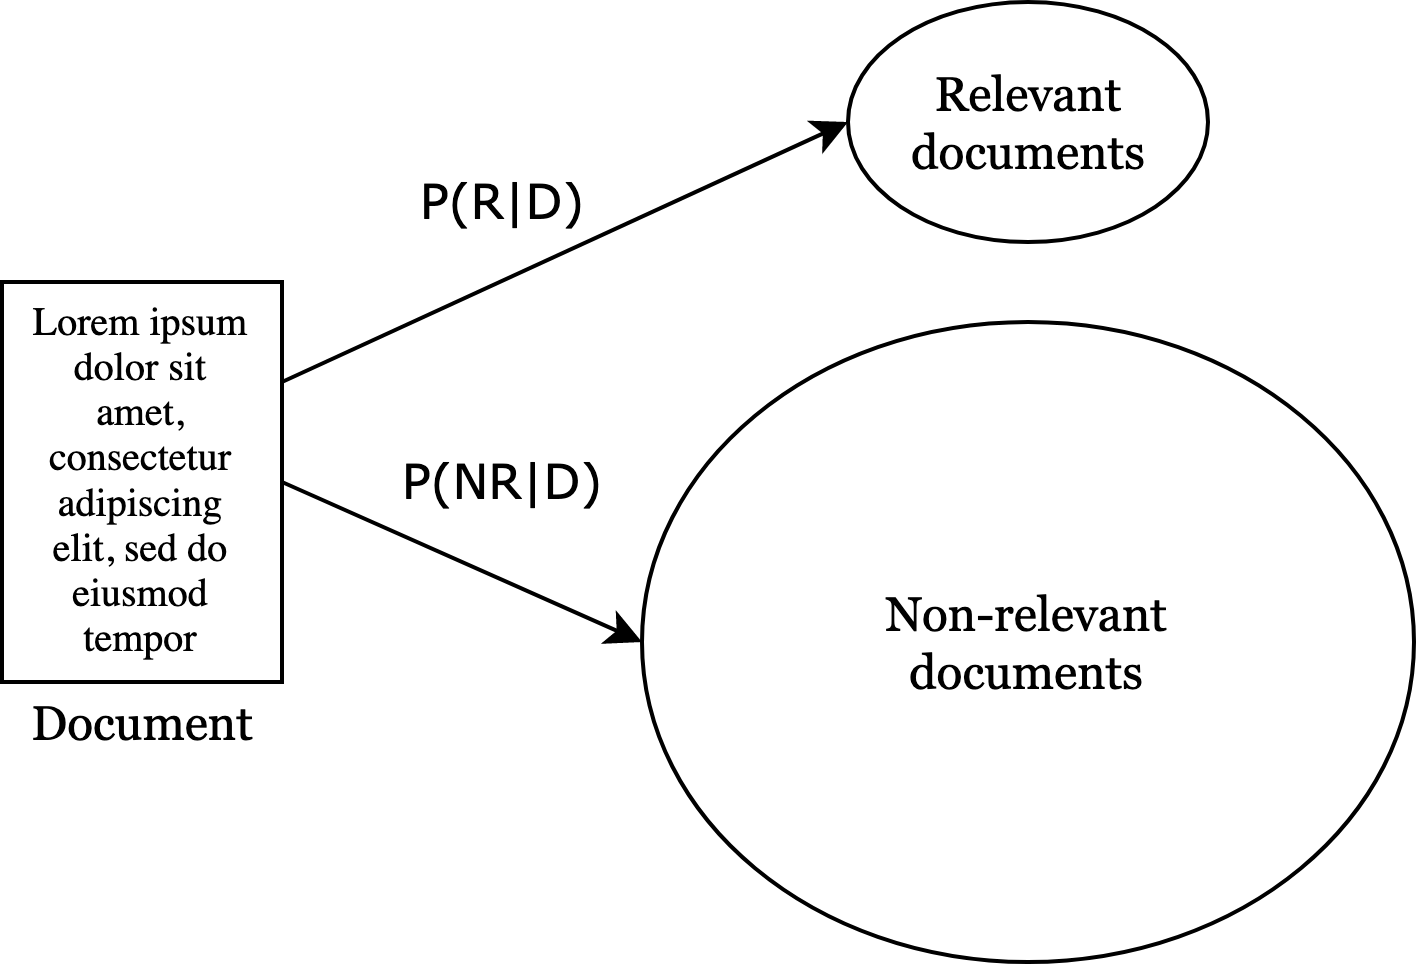
\includegraphics{images/probabilistic-ir.png}
\caption{Classifying a document as relevant or non-relevant\label{fig:probabilistic-ir}}
\end{figure}

\textbf{Probabilistic models} approach this problem from a probabilistic perspective. Using the well-known Bayes' theorem as their basis, they can lean on the robust foundation of probabilistic theory and apply many of its ideas to information retrieval. A general definition of the problem could be that there is a set of documents $D=\{d_1, ... d_n\}$ that should be categorized into two classes, relevant and non-relevant: $C=\{"R", "NR"\}$. To map the documents into those classes, a function $f$ is approximated $f: D \xrightarrow{} C$.

With Bayes' theorem this can modelled as a classification problem where the aim is to calculate the conditional probabilities of document being relevant $P(R|D)$ and non-relevant $P(NR|D)$, as shown in the Figure \ref{fig:probabilistic-ir}. It requires prior probabilities of any document being relevant $P(R)$ and non-relevant $P(NR)$, which could be measured by perhaps classifying some of the documents for a golden standard. The probability $P(D)$ is a normalizing constant that is the sum of all the probabilities of documents being relevant or non-relevant: $P(R)P(D|R) + P(NR)P(D|NR)$. To avoid calculating the conditional probability directly, we can turn this with Bayes' rule into Equation \ref{eq:bayes}.

\begin{equation}
\label{eq:bayes}
P(R|D)=\frac{P(R)P(D|R)}{P(D)}
\end{equation}
\vspace{-2pt}

A document would be classified as relevant when its conditional probability of relevancy would be higher than its non-relevancy: $P(R|D) > P(NR|D)$. This is referred to as the Bayes decision rule and the model Bayes classifier \cite{ir-in-practise}.

This model relies on the assumption that the documents can indeed be classified into relevant and non-relevant classes. While having a sound theoretical principle, in practise the relevancy of the documents is quite difficult to observe since it is subjective depending on the user. It will require advanced probabilistic models and a lot of data to accurately approximate users' perceptions of relevancy. Most large-scale search engines use probabilistic models and one of the most popular implementations is the Okapi BM25 model \cite{ir-in-practise}.

Codewebs avoids a part of this problem by using a user-specified seed set of documents that could be considered as the input for the search query. The system then retrieves the most relevant documents to that set with probabilistic modeling. This avoids having to write search queries but which might not be applicable to finding very specific patterns, only general approaches \cite{codewebs}. It is discussed in more detail in the Subsection~\ref{ssec:codewebs}.

An aspect we have omitted is the time and resources required to build the IR system. In most cases building your own search engine and probabilistic IR model might be too big of an undertaking unless it is the particular goal of the project. With CodeClusters, the building of a custom search engine for student code submissions was not considered as the particular aim of the project and instead already available libraries were used in the form of Apache Solr. 

\subsection{Vector space model}
\label{ssec:vsm}

As discussed in the previous subsection, one method to represent the documents is to use an algebraic model such as the vector space model. The simplicity of vector model has made it quite popular for all types of natural language applications beyond information retrieval to represent text documents. In vector space model, the documents and the search queries are represented as vectors in $s$-dimensional vector space, where $s$ is the number of unique terms. If the value of 1 was used when the document contained a specific term and 0 otherwise a binary term-frequency (TF) matrix would be produced, as shown in the Figure \ref{tbl:tf}.

\begin{table}[ht]
\begin{center}
\caption{Example binary TF matrix}
\label{tbl:tf}
\begin{tabular}{|c|c|c|c|}
\cline{1-4}
& \multicolumn{3}{ c|}{Documents} \\ \cline{2-4}
\hline
Term & $d_1$ & $d_2$ & $d_3$ \\
\hline % inserts single-line
\texttt{class} & 1 & 0 & 0 \\
\texttt{function} & 1 & 1 & 1 \\
\texttt{void} & 0 & 0 & 0 \\
$\vdots$ & $\vdots$ & $\vdots$ & $\vdots$ \\
\hline
\end{tabular}
\end{center}
\end{table}

Since this form is quite inflexible as it does not differentiate between how many times the term has appeared in a document, another possible weighting would be to use the raw term frequency count $tf_t=f_{t,d}$. Here $f_{t,d}$ is the frequency of the term $t$ in the document $d$. Other formats also exist. As discussed with the inverted index, this form is often non-optimal to use as such, which is why inverted indexes are used internally by the software.

The issue now becomes the ranking of the documents. A larger document that contains more terms will automatically rank higher than one that is smaller but which might be more relevant to the user. Therefore, a proportionate weighting is often added to this TF matrix in the form of inverse-document frequency.

\textbf{Inverse-document frequency (IDF)} is used to model the importance of the term relative to its occurrence in the documents. A term that can be found in all the documents will receive a IDF weight of 0, as it can not be used to distinguish between their differences. Its typical form is shown in the Equation \ref{eq:idf}.

\begin{equation}
\label{eq:idf}
idf_t=\log\frac{N}{n_t}
\end{equation}
\vspace{-6pt}

Where $N$ is the number of the documents, $n$ the number of documents the term $t$ appears in and $t$ the term in question. The TF matrix and IDF weights are often combined into one as the TF-IDF matrix, which is the TF weights multiplied by the IDF scores of the terms.

This format works relatively well for code as it does for text. One problem with the generation of a TF matrix is the pruning and normalization of the terms, which is amplified by natural language's ambiguity with synonyms and spelling errors. With code, the tokens are much less ambiguous although some tokens, like \texttt{while}-constructs, can be written in multiple ways.

A much bigger problem of the TF-IDF matrices is that the frequencies are unordered relative to how they occur in the documents, resulting in the loss of the original sequence. Hence this format is often called the "bag of words" model and it makes distinguishing structural patterns from the documents difficult. Another problem is every term having an equal importance in the weighting, whereas the teacher would probably rate a higher-level structure such as \texttt{class} or \texttt{function} as more important than variable assignments.

Having now enhanced the ranking of the documents, we must also find a way to score them in relation to the search query. This can be done with a similarity measure, of which the most popular one for vector space models is cosine similarity.

\textbf{Cosine similarity} calculates the cosine of the angle between two vectors which produces a value between 0 and 1, where 0 indicates orthogonality and 1 the exact same angle. This makes it very simple to use as it does not have to be otherwise normalized. Another benefit of cosine similarity is that since vectors of documents with a lot of terms become longer than the smaller documents', cosine similarity is not effected by their length. This proportionality mitigates one of the weaknesses of TF representation.

Scoring similarities for each document-query pair produces a similarity vector with which the documents could be ranked. On the other hand, if we scored similarities between each document pair we would create a similarity matrix as previously shown in the Equation \ref{eq:sim-matrix}, consisting of real numbers between 0-1 which is symmetric and has diagonal values of 1. This is the same format used in similarity detection as described in more detail in the Section \ref{sec:sim-detection}.

While we could save space by using an inverted index representation of the matrices, a problem often arises with terms that are popular but which do not offer a lot of predictive power. This becomes a problem even with a moderately sized dataset which makes computation inefficient. To reduce the dimensionality of the matrix we would want to remove those term vectors that do not improve our ranking.

\textbf{Singular value decomposition (SVD)} of $m \times n$ matrix \textbf{M} are the three matrices $\textbf{U}$, $\Sigma$ and $\textbf{V}^{T}$ as shown in the Equation \ref{eq:svd}. Here \textbf{U} and $\textbf{V}^{T}$ are two orthogonal matrices of size $m \times m$ and $n \times n$ and $\Sigma$ a diagonal matrix of size $m \times n$ with all the singular values of \textbf{M} as its diagonal values. In our case the $m$ would be the number of terms and $n$ the submissions \cite{intro-to-ir, mmds-2014-ullman}.

\vspace{-6pt}
\begin{equation}
\label{eq:svd}
\textbf{M}=\textbf{U}\Sigma\textbf{V}^{T}
\end{equation}
\vspace{-10pt}

When SVD is used for dimensionality reduction the aim is to decrease the size of the matrix \textbf{M} by removing the singular values that are very low relative to the others. This makes for a lot more efficient computation especially with large sparse matrices. In truncated SVD, which is what CodeClusters uses, an approximation of $\widetilde{\textbf{M}}=\textbf{U}_t\Sigma_t\textbf{V}^{T}_t$ is used where $t$ are the largest singular values of $\Sigma$. This is similar to Principal Component Analysis (PCA) where the least variance producing eigenvalues are discarded but in this case the data does not need to be centered thus it works well with the sparse TF-IDF matrices. Using SVD for TF matrices, such as TF-IDF, is often referred to as Latent Semantic Analysis (LSA) which is the finding of latent, underlying, relationships between the terms \cite{intro-to-ir, mmds-2014-ullman}.

In the Section~\ref{sec:sim-detection} similarity detection is discussed in more detail and in the Section~\ref{sec:clustering}, unsupervised learning methods to cluster the similarity or distance matrices.
